\section{Méthodes de positionning}
Dans cette partie, il s'agira de faire une liste des méthodes d'indoor positionning.
Ces méthodes sont divisées en deux grandes catégories. Premièrement les range-based, à savoir les méthodes basées sur des mesures de distances entre un émetteur et un récepteur. Deuxièmement les range-free, les méthodes reposant sur les échanges d'informations de connexion entre noeuds.


\subsection{Méthodes range-based}


\subsubsection{Méthode basée sur la force du signal}


Il existe deux méthodes qui s’appuient sur la puissance du signal reçu.
\medskip
\\
La première repose sur une corrélation directe entre la puissance et la distance.
Dans cette méthode la puissance mesurée au niveau du tag est représentative de la distance vis-à-vis des antennes de références. 
Différentes équations permettent de modéliser le comportement du canal et ainsi, quantifier les atténuations du signal en fonction de la distance parcourue. 
Cette méthode est très calculatoire car elle se base sur des résolutions d'équations complexes.
\medskip
\\
La seconde quant à elle est basée sur un algorithme de comparaison. 
En amont de la localisation, il est nécessaire de procéder à une phase de fingerprinting, de relevé en différents points des puissances des différentes anchors pour constituer une base de données. 
Cette base de données ainsi créée permettra lors de la phase de localisation de comparer les puissances reçues avec celles préenregistrées et on pourra en déduire la position estimée du tag.
\begin{figure}[h!]
    \centering
    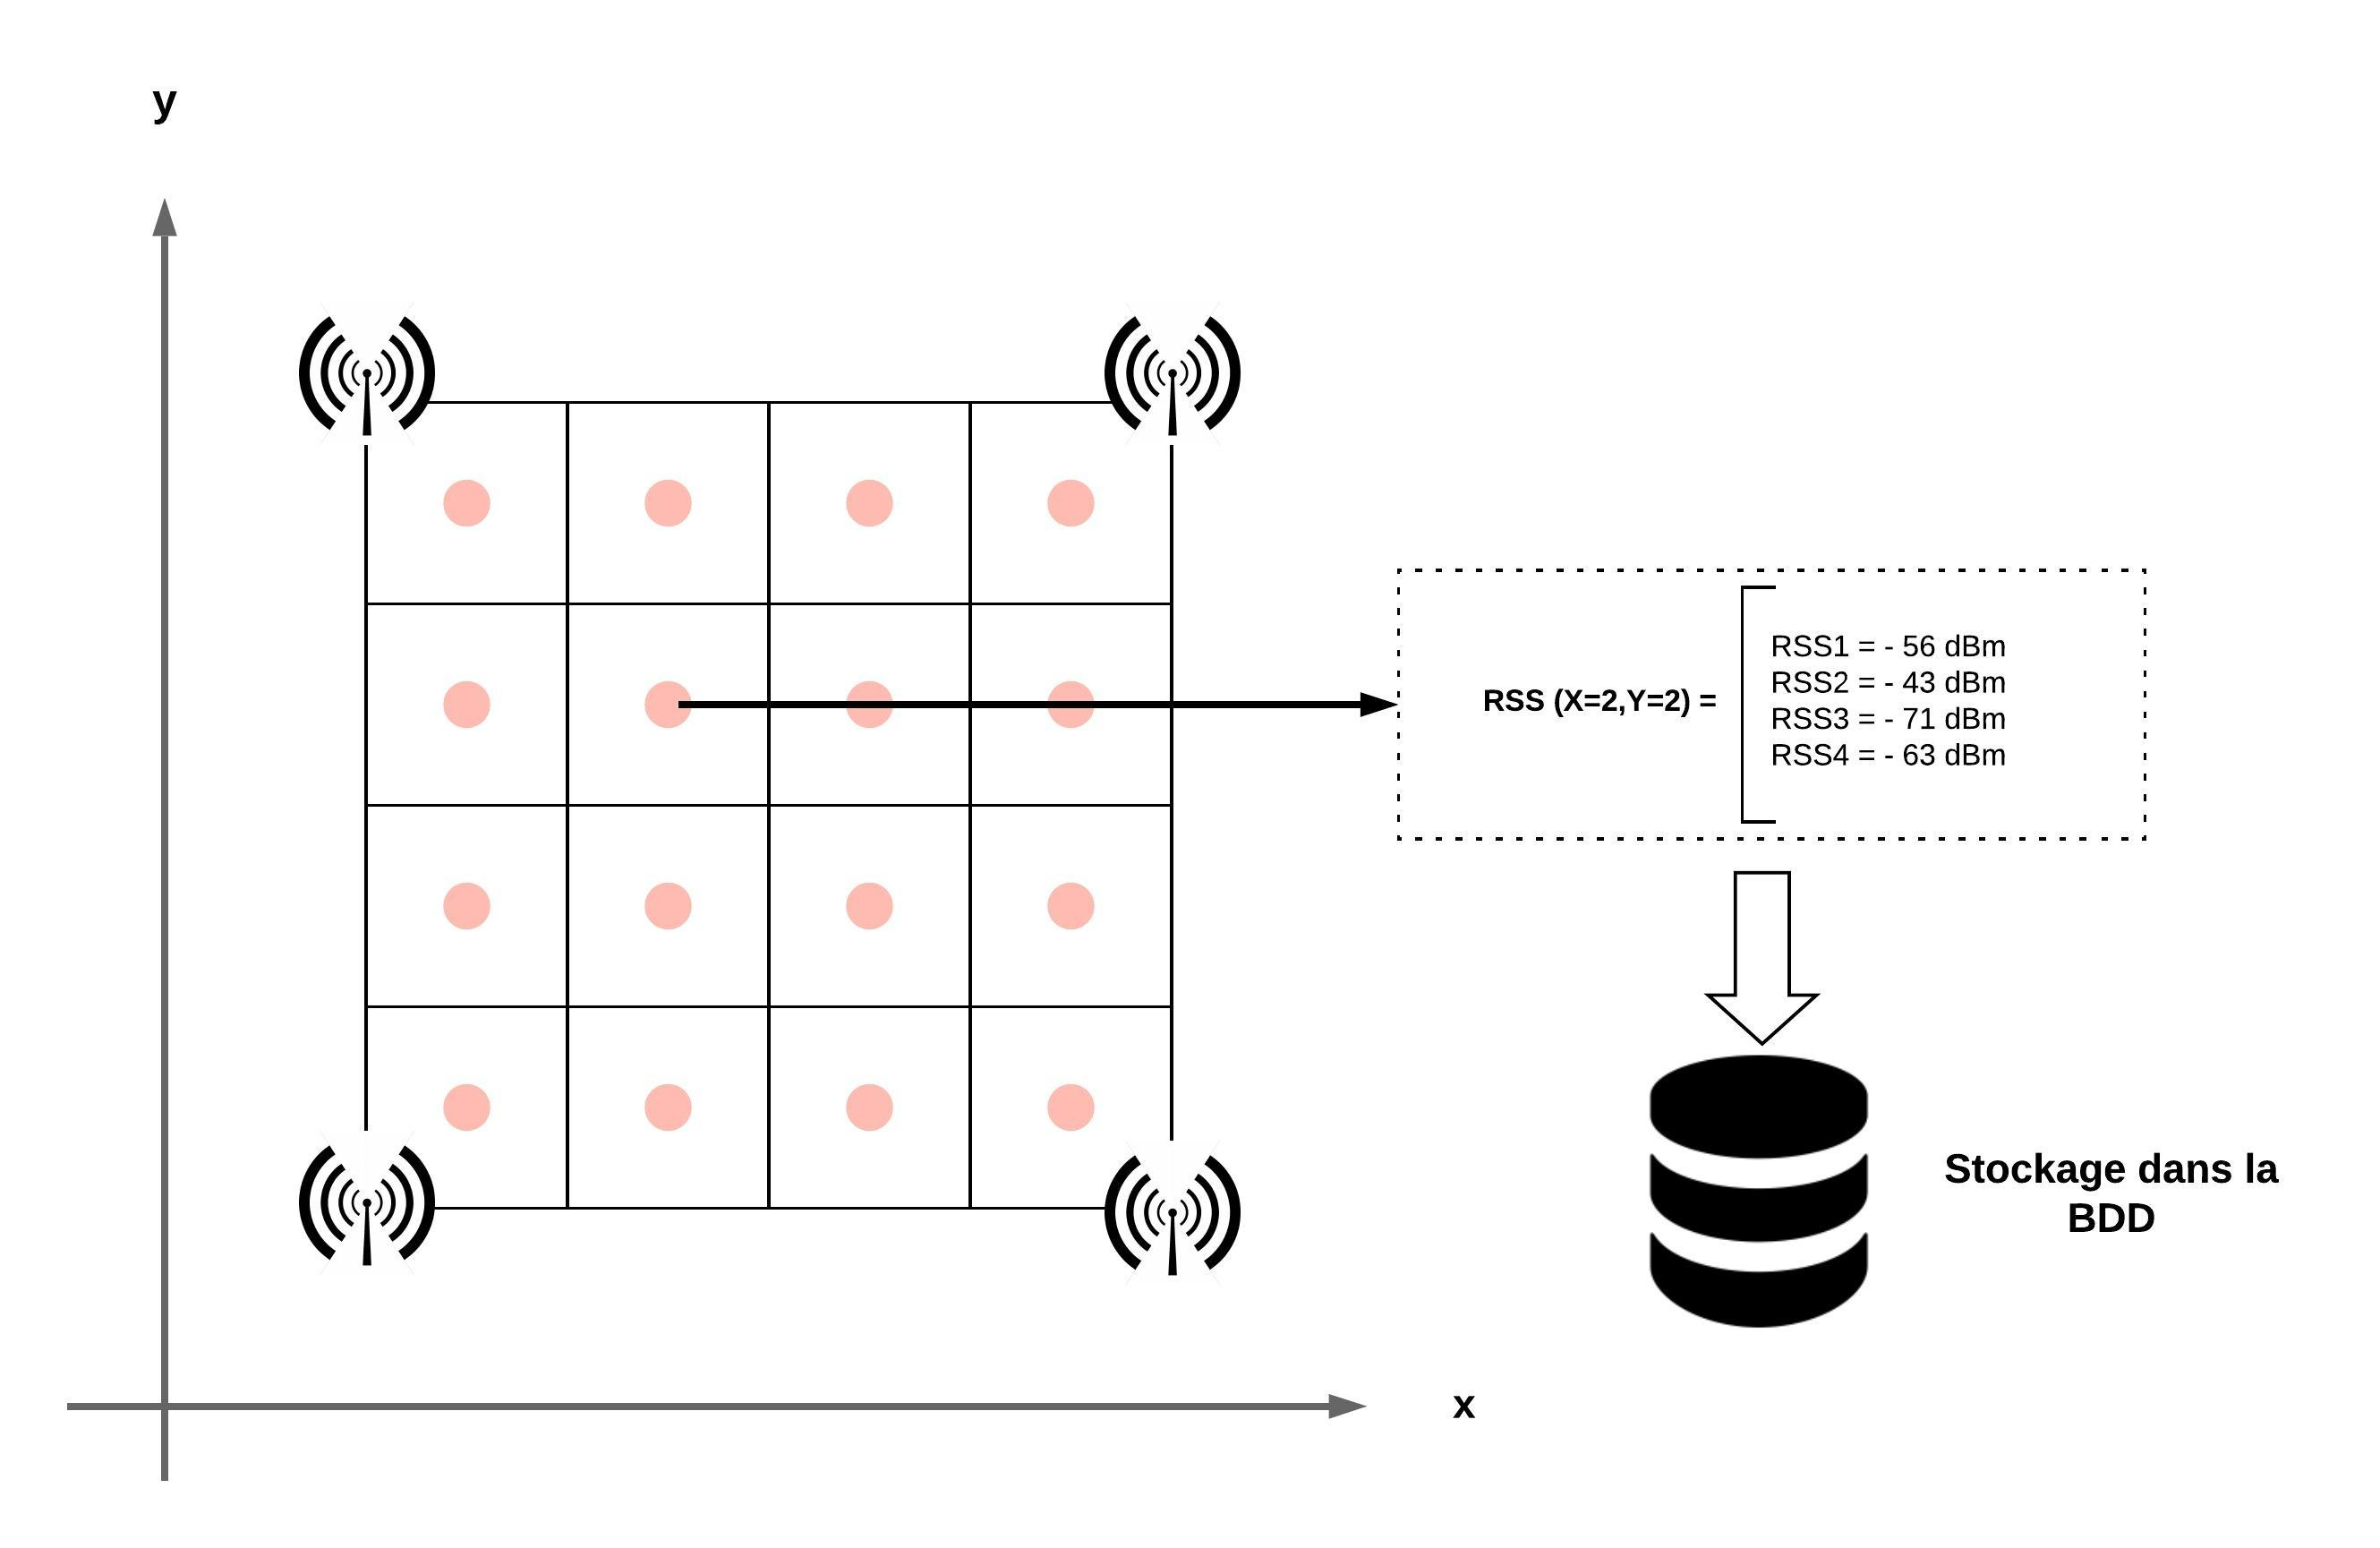
\includegraphics[width=1\textwidth]{\pathMeth/RSS.jpeg}
    \caption{Méthode de calcul de position basé sur les mesures de forces de signaux.}
\end{figure}
Le principal avantage de ces techniques est la rapidité d'implémentation. En effet, celles-ci ne nécessitent que très peu de calcul et sont facilement adaptables.
\medskip
\\
Cependant, le défaut majeur de cette technique est qu'il est nécessaire d'avoir une zone parfaitement neutre, car les interférences faussent les calculs.
La deuxième méthode quand à elle nécessite un investissement en temps relativement important en cas d’implémentation dans un nouvel environnement, et n’est donc adaptée que dans le cadre d’une utilisation dans un domaine relativement stable.


\subsubsection{Méthodes basées sur des mesures d'angle}

La méthode AOA, pour Angle-of-Arrival est une méthode de localisation qui se base sur la mesure des angles d'arrivées de signaux d'au minimum deux anchors par rapport à un tag.
Après détermination des angles de réception, la position du tag est obtenue par l'intersection des différentes droites et par un système de triangulation.
\medskip
\\
Cette méthode nécessite bien évidemment d'être en vue directe du tag auquel cas les angles ne pourraient être établis, mais la précision de cette méthode est de l'ordre de la vingtaine de centimètres.
\begin{figure}[h!]
    \centering
    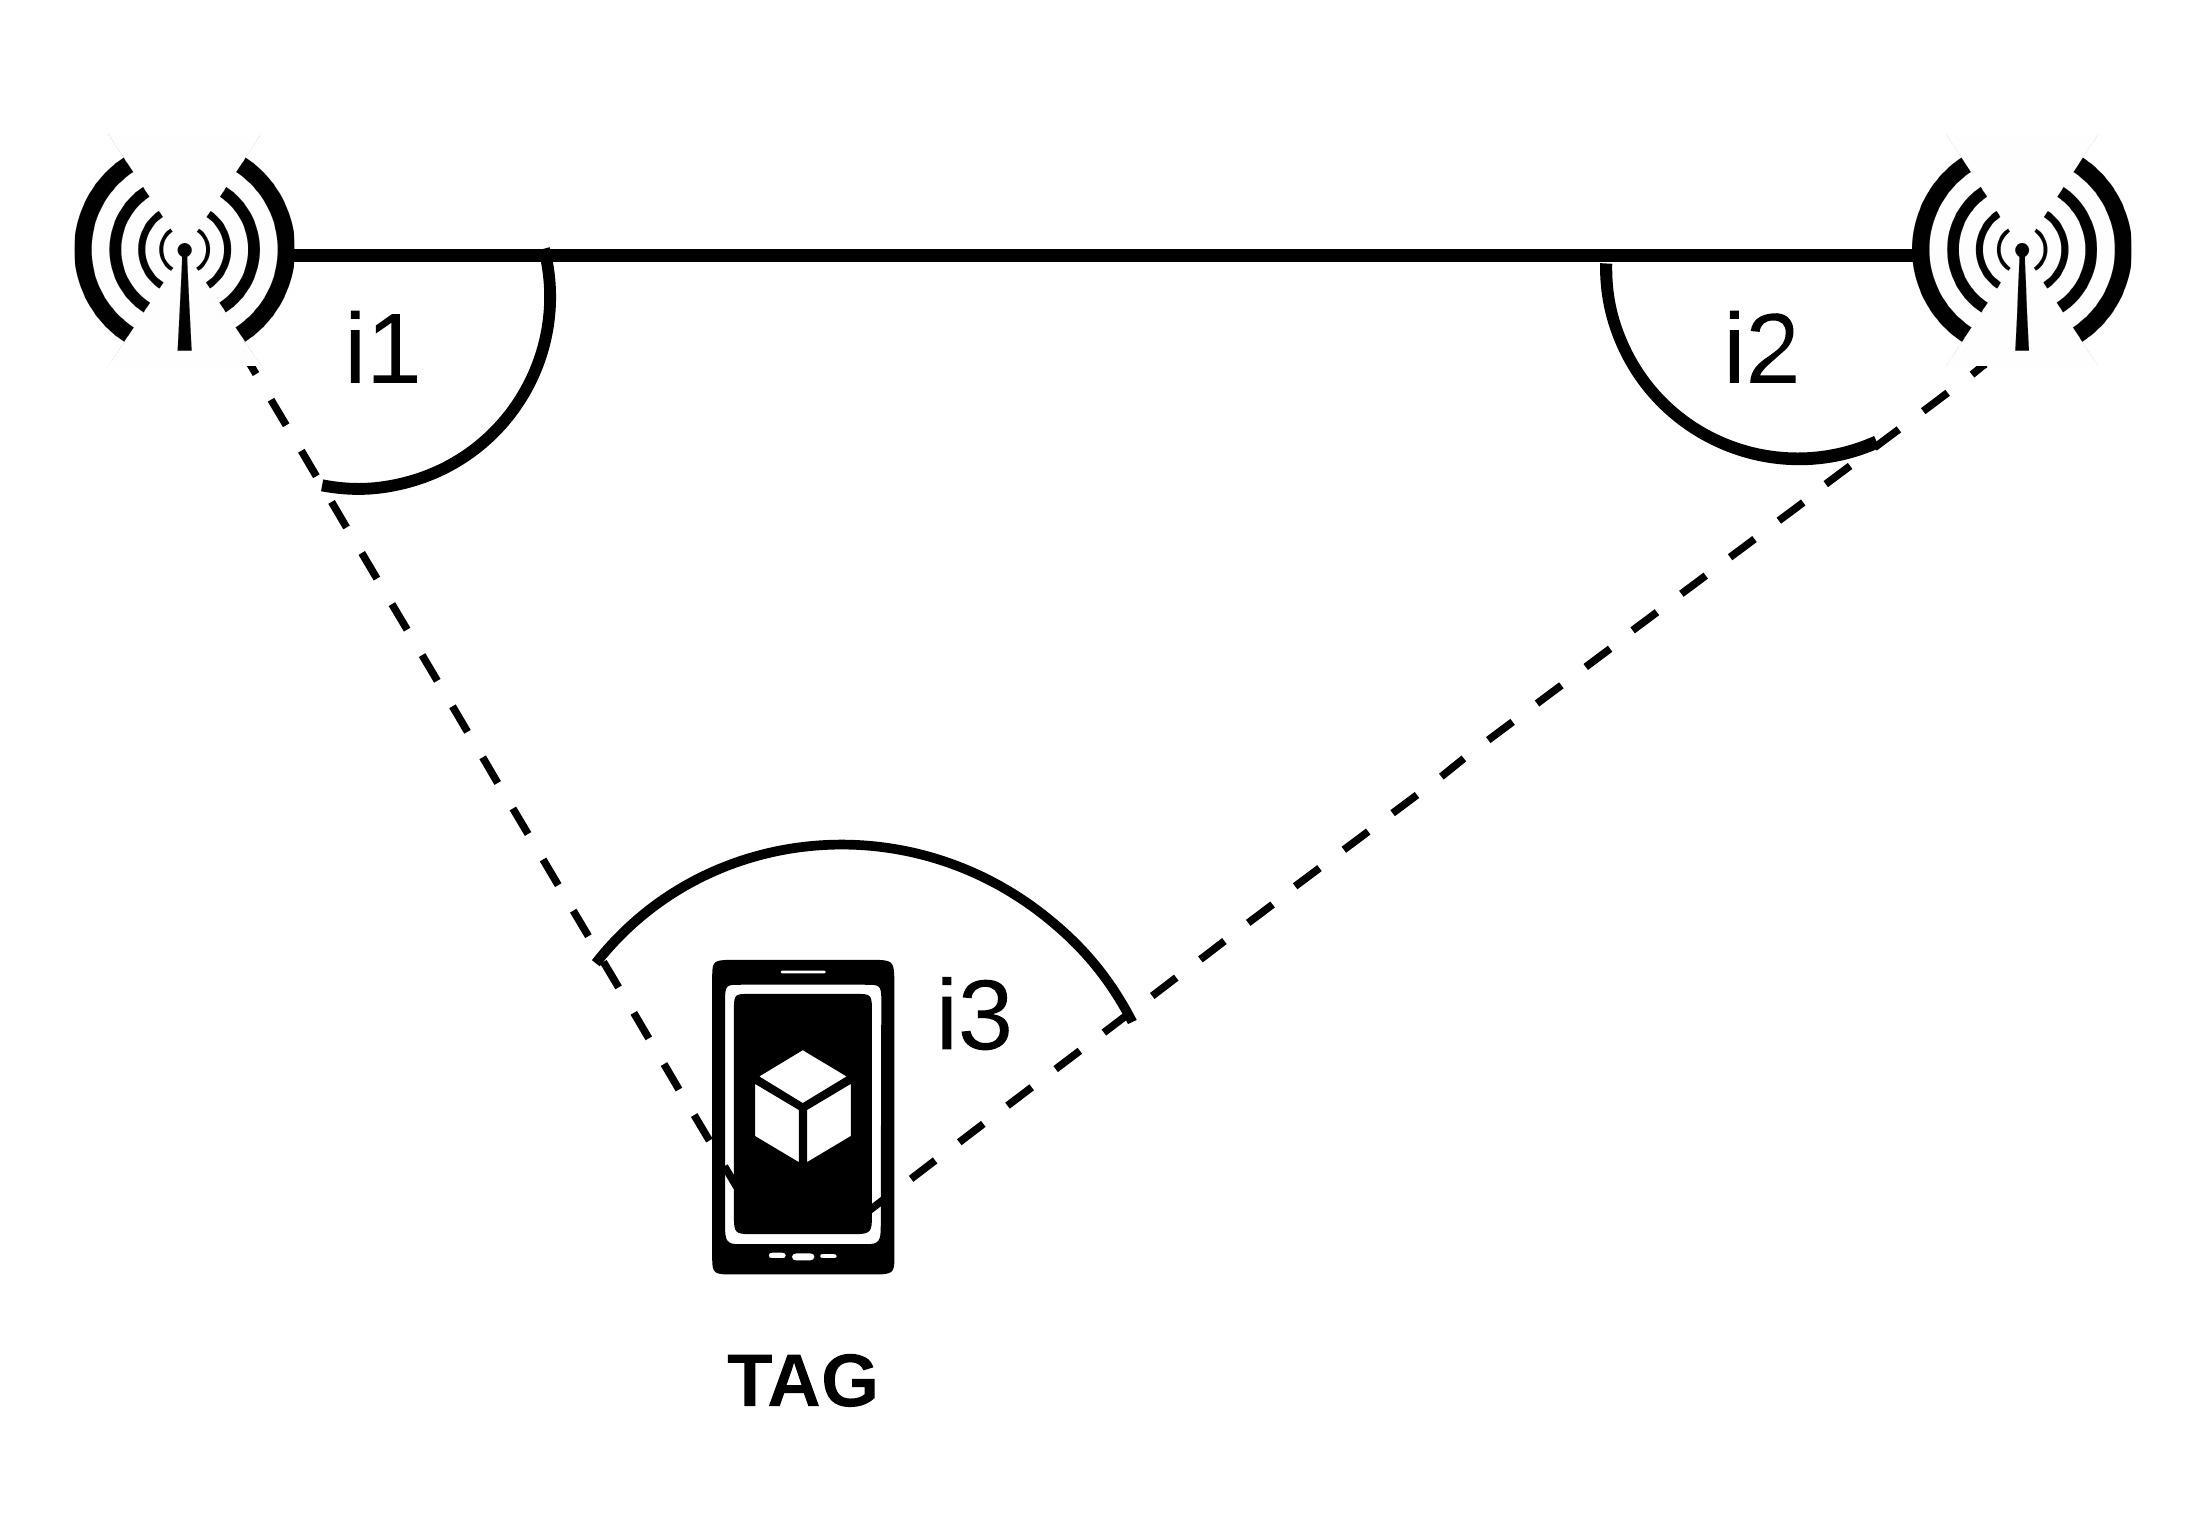
\includegraphics[width=0.6\textwidth]{\pathMeth/angle.jpeg}
    \caption{Méthode de calcul de position basée sur les mesures d'angle.}
\end{figure}


\subsubsection{Méthodes basées sur des mesures de temps}

La méthode TOA, pour Time-of-Arrival est une méthode de localisation qui se base sur la mesure du temps d'arrivée d'un signal à un tag.
Ce procédé s'appuie sur le temps de propagation d'un signal, entre l'émission par le tag à l'instant "Ti" et la réception au niveau de l'anchor à l'instant "Tf".
\medskip
\\
On peut diviser cette méthode en sous-méthodes.
\begin{itemize} 
    \item la méthode One-Way TOA
    \item la méthode Two-way TOA
\end{itemize}
Dans cette première configuration le temps de propagation des ondes de chaque anchor peut être corrélé à une distance d = c * (Tf – Ti), vis-à-vis du tag où c est la vitesse de propagation de l'onde dans l'air.
Leur position dans l’environnement étant connue, l’utilisateur se repère alors quelque part sur le cercle de rayon d et d’origine l’antenne en question. Répéter cette opération pour un minimum de trois anchors permet d’extraire une position en espace 2D (à l’intersection des 3 cercles alors construits). Le procédé est dit de « trilatération ».
\begin{figure}[H]
    \centering
    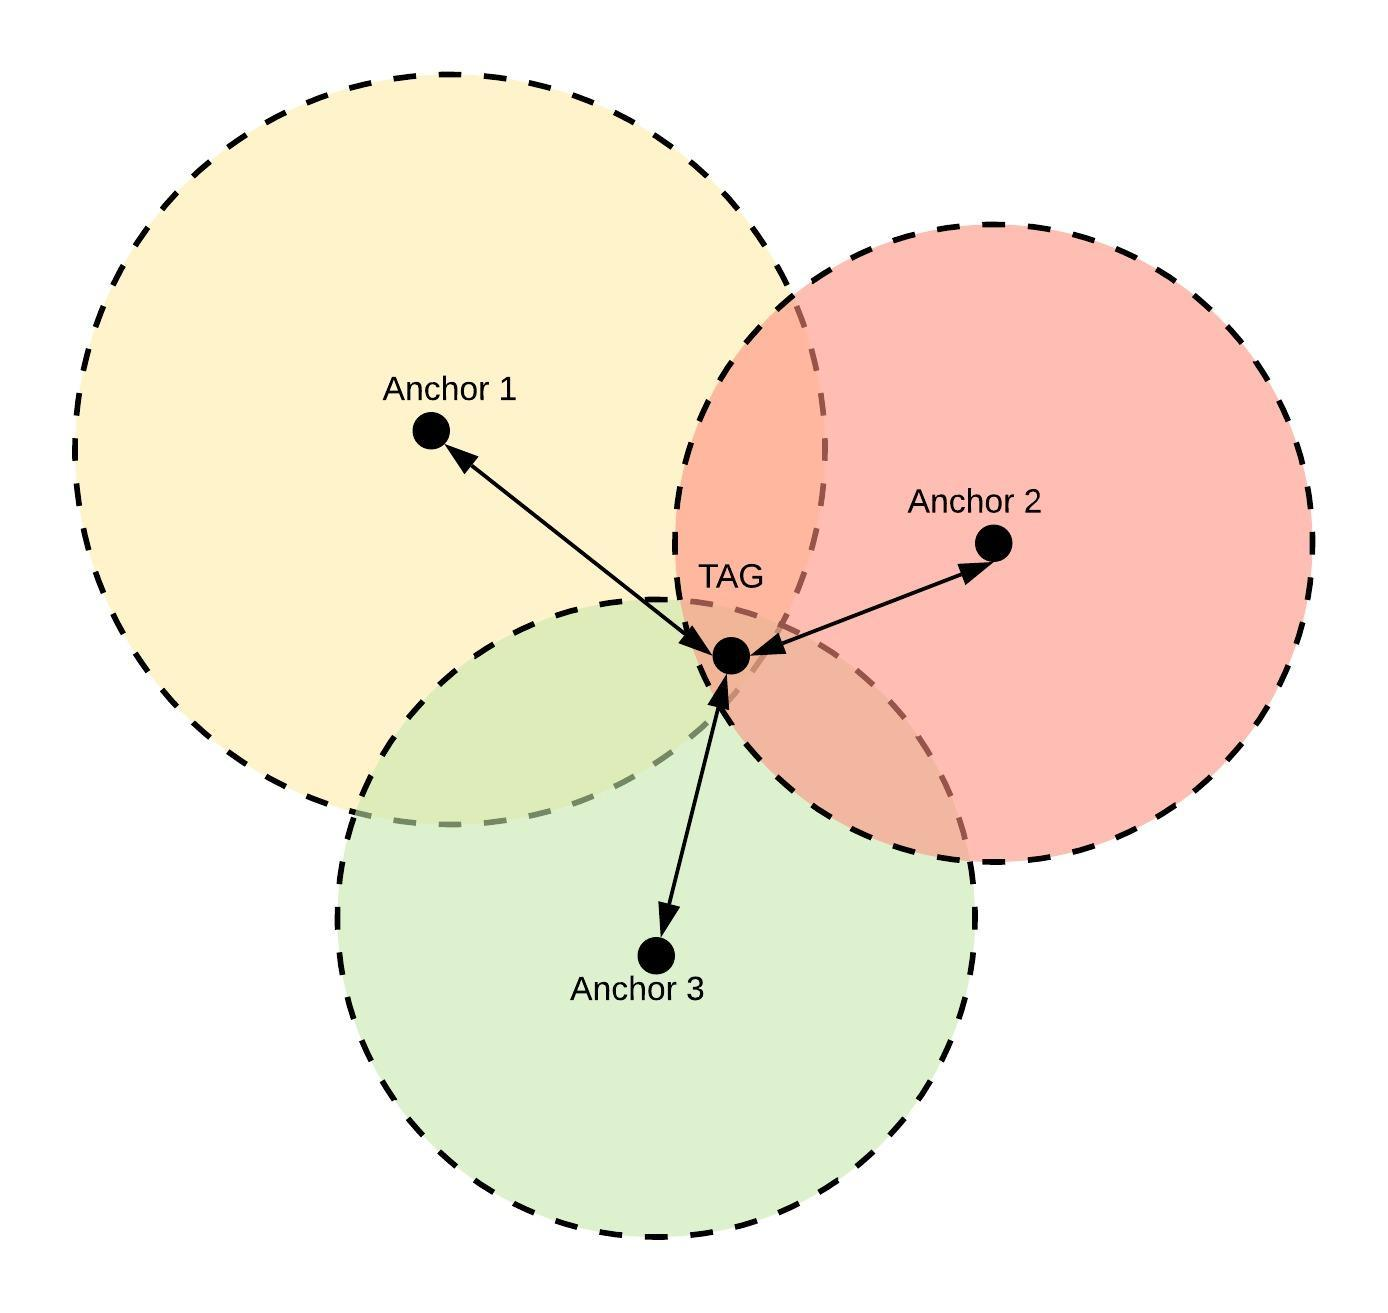
\includegraphics[width=0.6\textwidth]{\pathMeth/time.jpeg}
    \caption{Méthode de calcul de position basé sur le One-way TOA.}
\end{figure}
\newpage
Pour la deuxième configuration, nous sommes dans le cas où une anchor envoie un message et l'anchor réceptrice lui retransmet des informations en retour. 
Il y a ici une nécessité de synchronicité de temps entre les nœuds pour ne pas fausser les données.
\\
Nous pouvons prendre comme exemple le cas suivant : \\
\begin{itemize} 
    \item L’anchor envoie un message au tag et enregistre à quel temps le message est transmis (Ti)
    \item Le tag reçoit le message et le renvoi une réponse à l’anchor.
    \item L’anchor enregistre le temps du moment de la réception du message retourné (Tf)
    \item L’anchor calcule la différence de temps qui correspondra au temps de l’aller-retour du message (T = Tf-Ti)
    \item L’anchor en déduit la distance (d) connaissant la vitesse de propagation dans l’air du message (c) 
    \item d = c * T/2
\end{itemize}
Ces méthodes sont encore une fois précises, mais nécessitent qu'il n'y ait pas d'obstacle entre les anchors et le tag. De plus, dans la deuxième méthode il est nécessaire d'avoir une synchronicité entre les anchors (noeuds).


\subsubsection{Méthodes basées sur des mesures de différences de temps}

La méthode TDOA, pour Time-Difference-of-Arrival est une méthode de localisation qui se base sur la mesure de la différence des temps d'arrivés d'un signal à des anchors.
Ce procédé est très similaire aux méthodes de ToA, mais permet de s’affranchir de la synchronisation temporelle entre émetteur et récepteur, toutefois la synchronisation temporelle entre les anchors doit demeurer extrêmement précise.
En pratique une anchor maîtresse est donc en charge de communiquer son horloge aux autres anchors à proximité. 
Par la suite le tag émet à intervalles réguliers de courts messages diffusés en broadcast. 
La différence entre les temps d’arrivées du signal au couple de capteurs traduit une différence de distance entre l’objet à localiser et ce même couple. Celui-ci se situe alors sur une hyperbole ayant pour foyer les deux récepteurs. 
Sa position exacte est finalement obtenue après réitération du processus, à l’intersection des hyperboles construites.
\begin{figure}[h!]
    \centering
    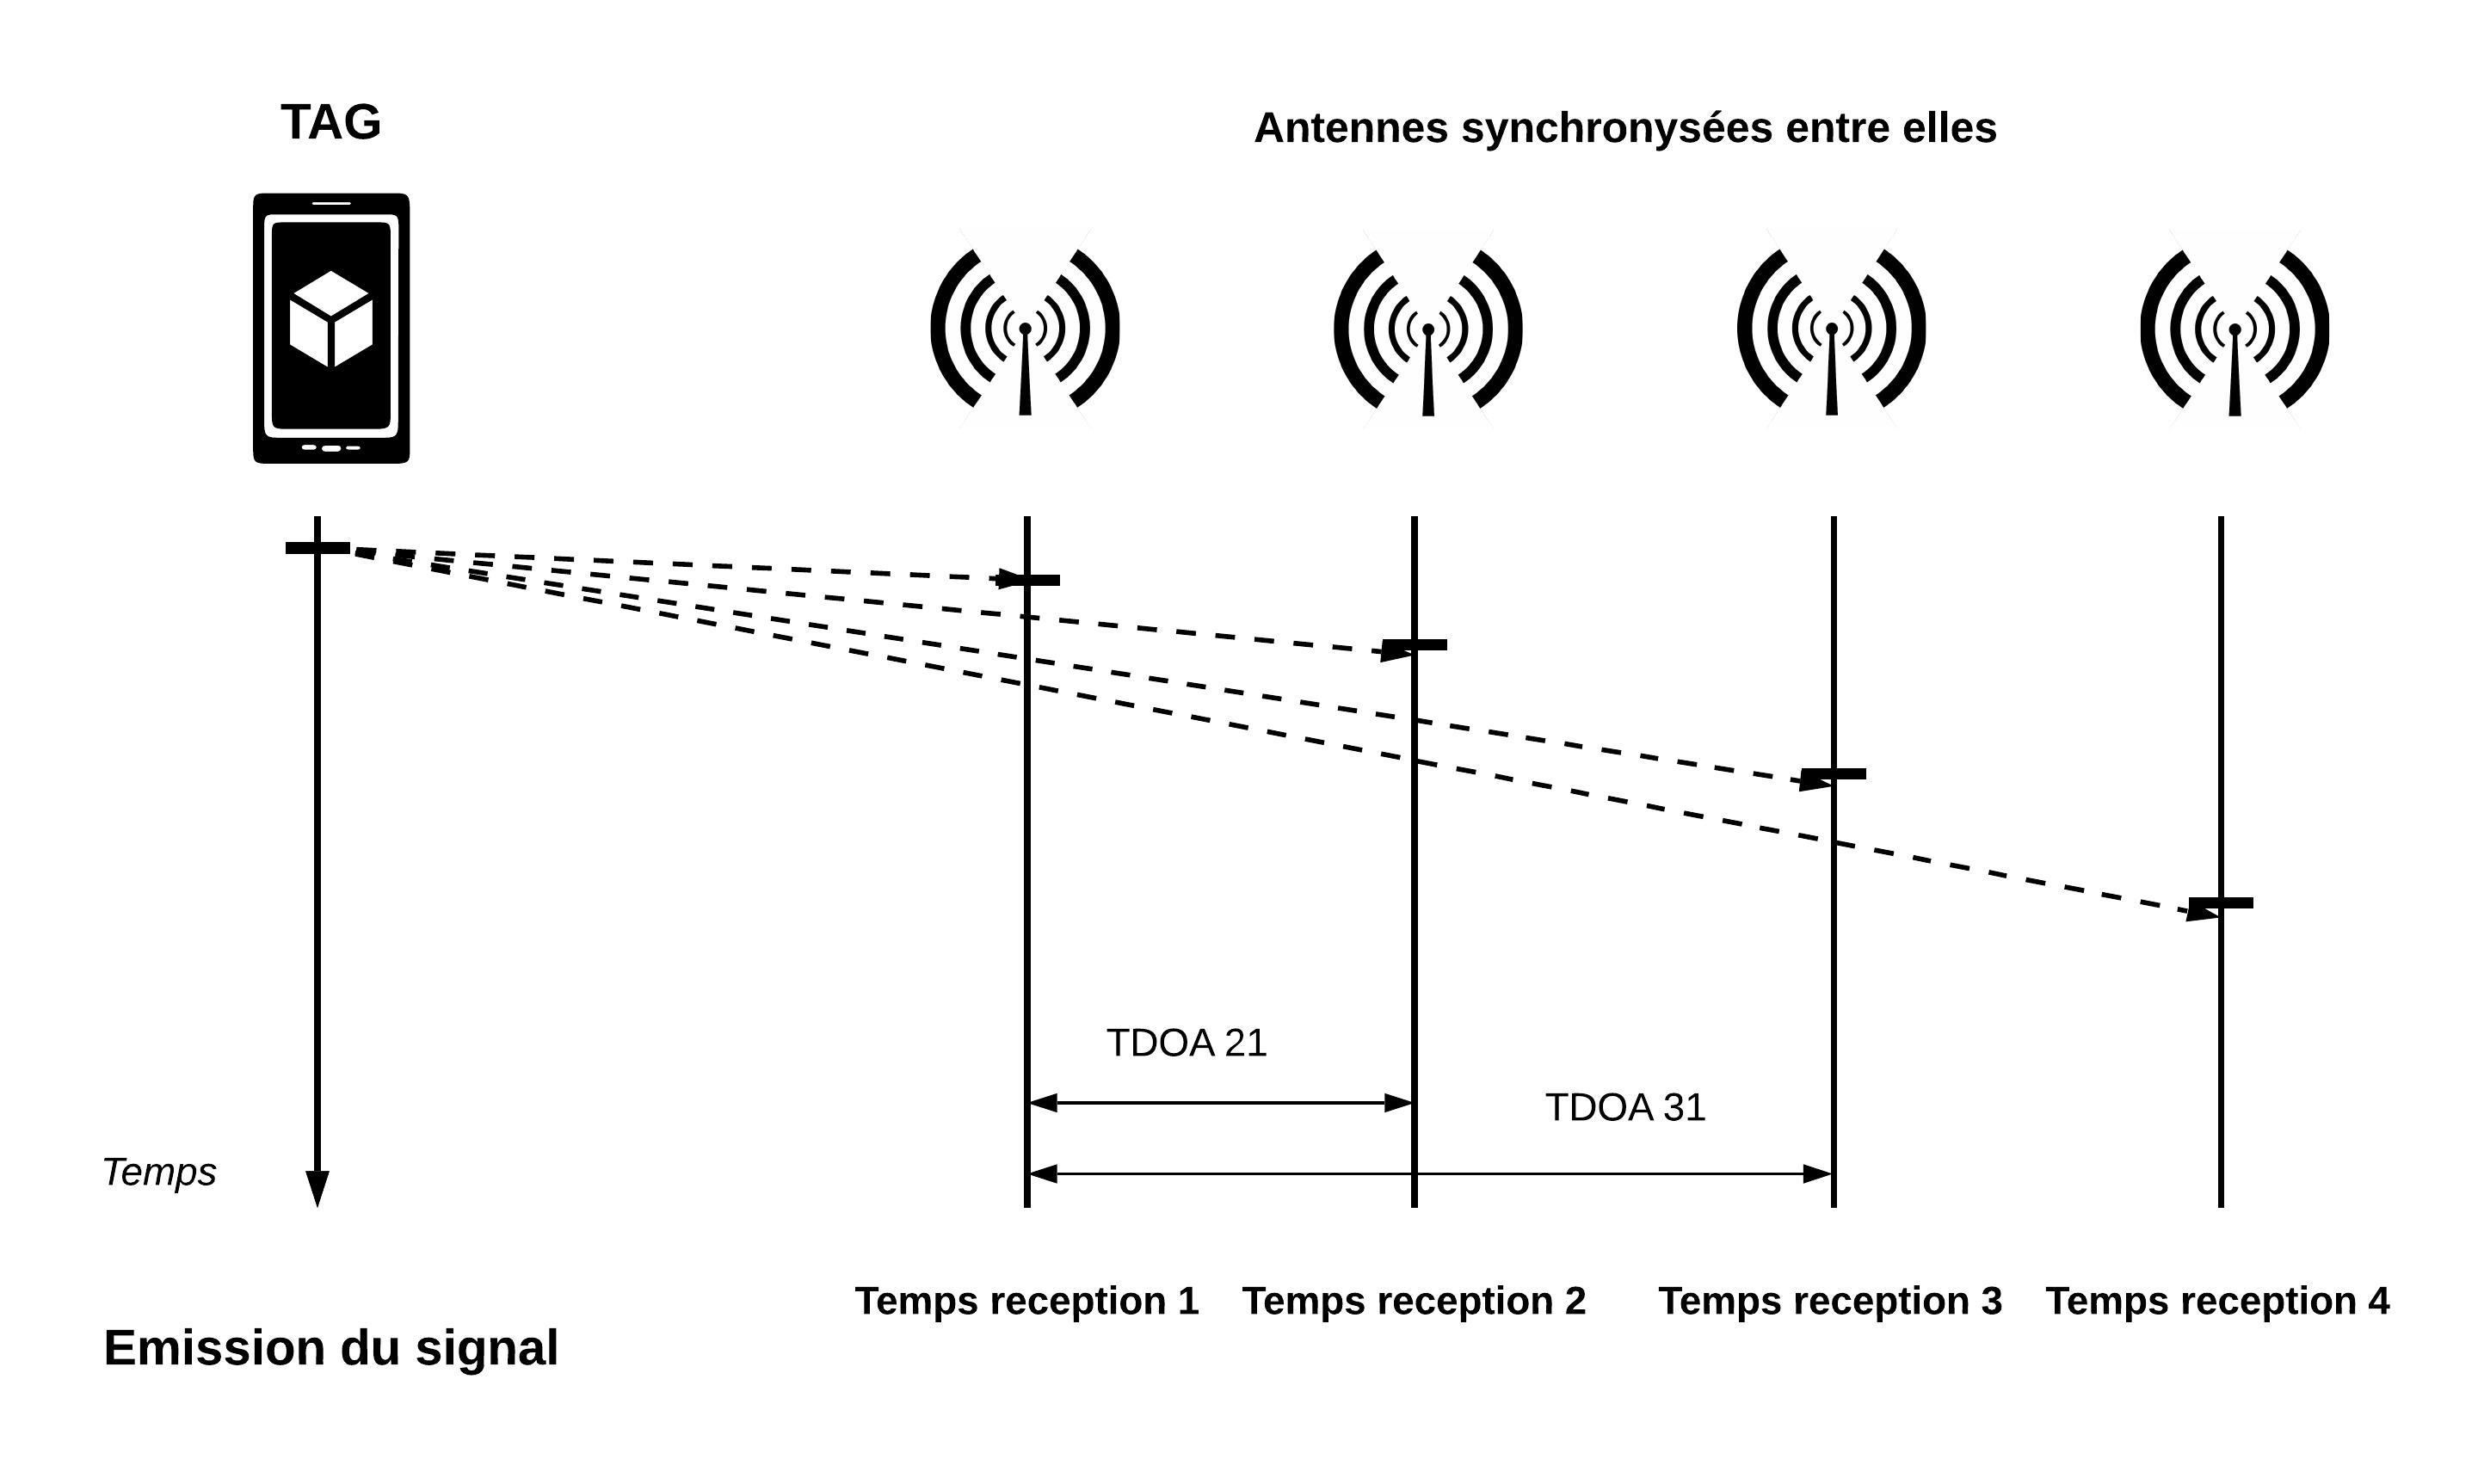
\includegraphics[width=1\textwidth]{\pathMeth/TDOA.jpeg}
    \caption{Méthode de calcul de position basée sur le TDOA.}
\end{figure}


\subsection{Méthodes range-free}

Plus économique du point de vue du matériel que les méthodes range-based, les méthodes range-free se basent sur toutes les informations de connectivité en lien avec la porté radio. Elle ne nécessite donc pas l'achat supplémentaire d'anchor par exemple.
Il en existe deux principales méthodes : DV-hop et l'intersection des signaux.


\subsubsection{Méthode DV-hop}

La méthode DV-hop pour distance vecteur hop est la méthode la plus courante dans la famille des méthodes range-free.
Cette technique se base sur le nombre de sauts séparant les noeuds d'un réseau.
Prenons l'exemple suivant : 
\begin{figure}[h!]
    \centering
    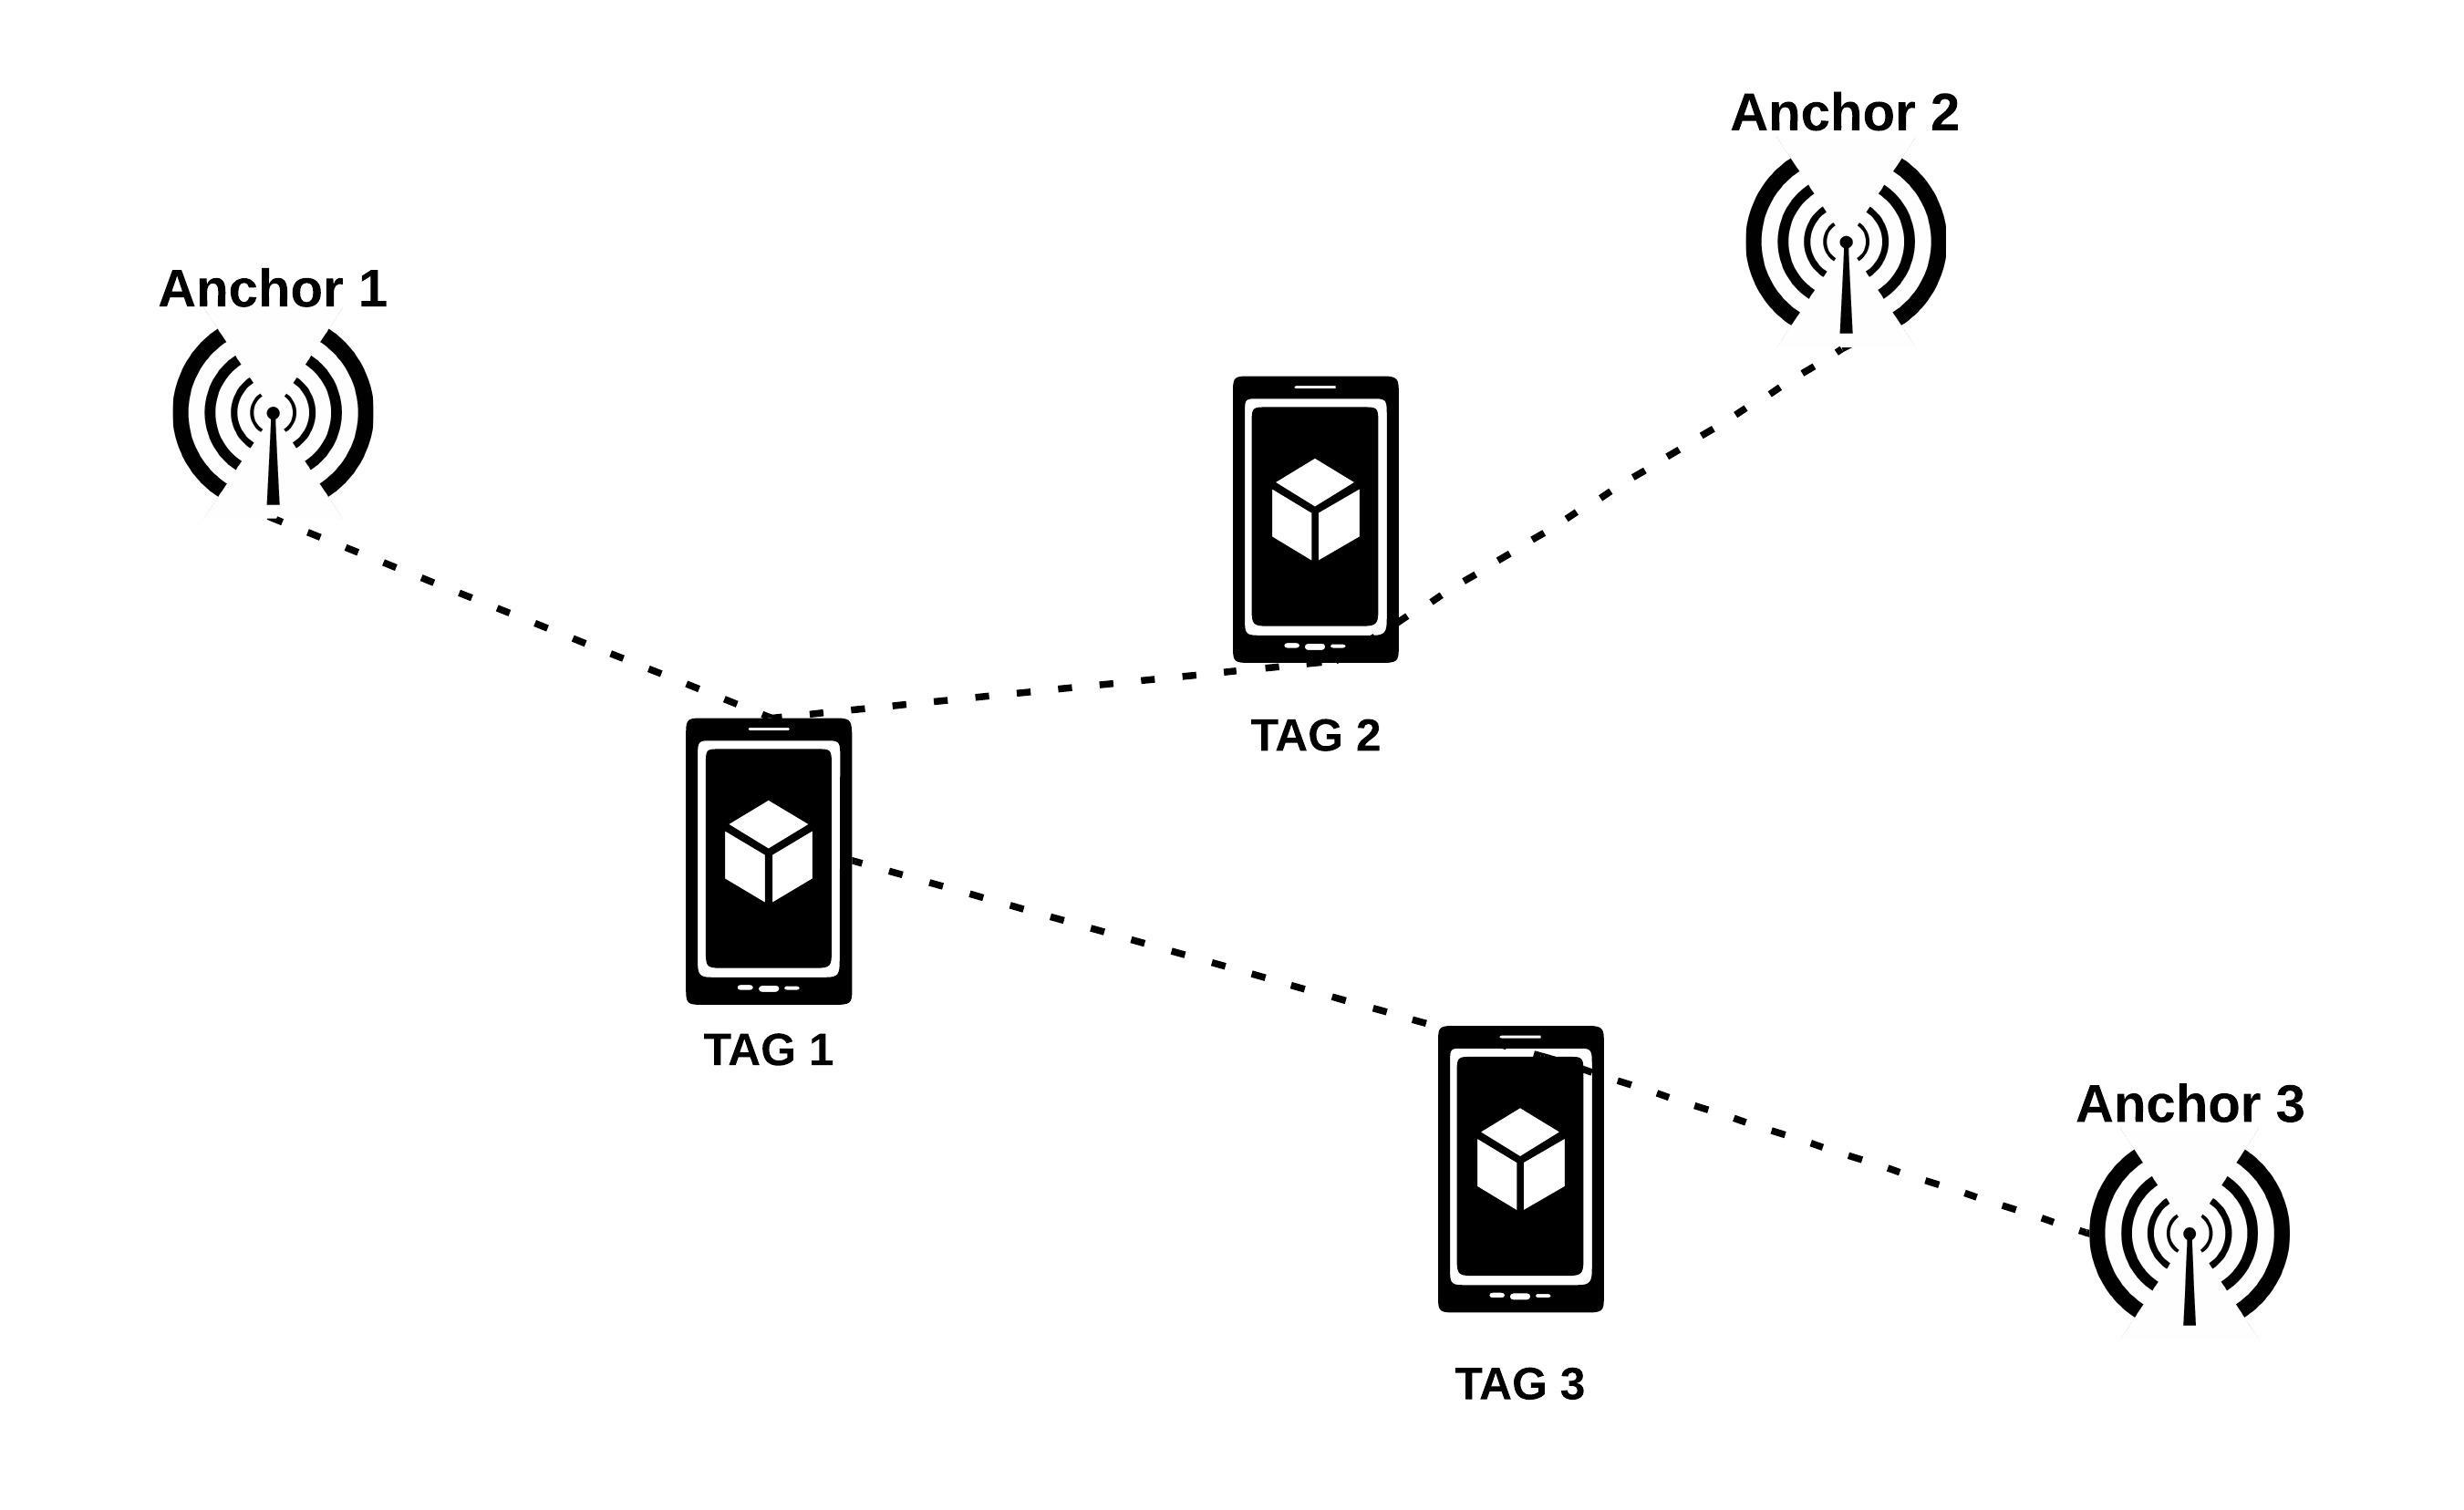
\includegraphics[width=0.6\textwidth]{\pathMeth/DV.jpeg}
    \caption{Méthode DV-hop}
\end{figure}
Nous avons ici trois tags et trois anchors, à l'aide d'un protocole de diffusion, chaque anchor va diffuser sa position à tous les tags.
L'anchor 1 connaîtra donc la position des anchors 2 et 3 et elle sera aussi qu'elle est à trois sauts de ces dernières.
À partir de là, toutes les anchors vont calculer la distance moyenne par saut, moyenne qui sera utilisée comme étalon de distance pour les sauts de tous les autres noeuds et on pourra ainsi trouver la position d'un tag par rapport aux anchors qui l'entoure.
Il faut savoir que cette technique est très peut précise, on parle d'ici d'une marche d'erreur de 30 pour cent.


\subsubsection{Méthodes d'intersection de signaux}

Nous avons ici une multitude d'anchors formant une zone de localisation. Chaque anchor va connaître les anchors avoisinantes, leur position et leur portée.
Le tag pourra ainsi évoluer parmi les anchors et sa position sera trouvée par l'intersection de deux ou trois anchors les plus proches.
\begin{figure}[h!]
    \centering
    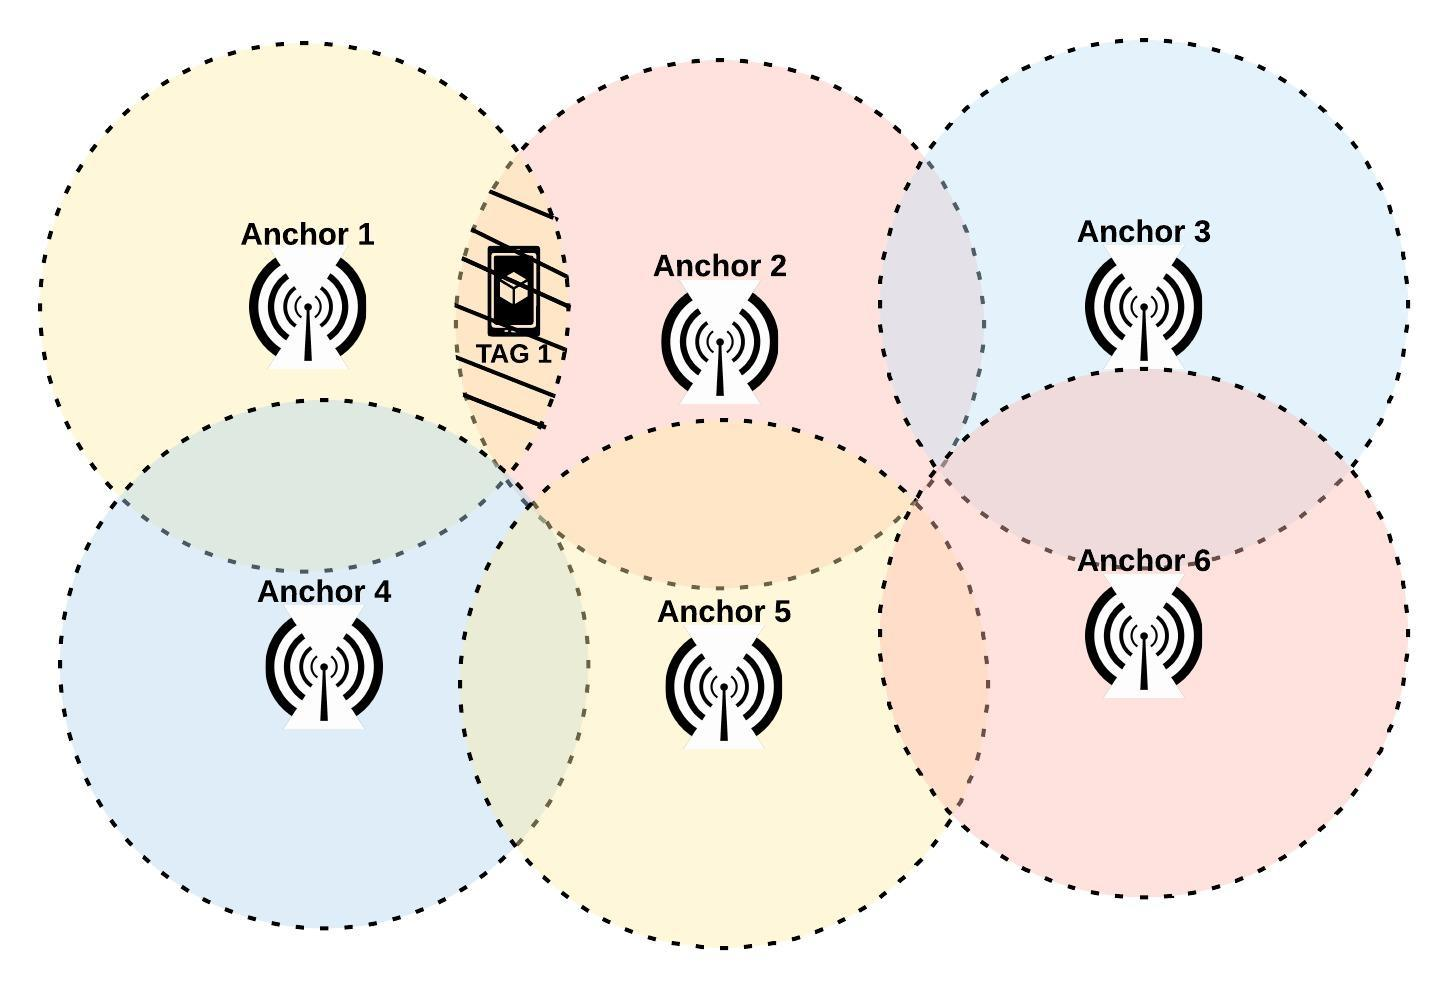
\includegraphics[width=0.8\textwidth]{\pathMeth/inter.jpeg}
    \caption{Méthode DV-hop}
\end{figure}
Cette technique est assez précise bien que la précision varie selon la portée des anchors ainsi que leur nombre dans la zone de détection.


\subsubsection{Élargissement}

Bien évidemment, il existe d'autres méthodes range-based même si la grande majorité d'entre elles restent théoriques.
Avec l'évolution actuelle, des puissances de calcul et le développement des algorithmes de machine-learning de nouvelles méthodes voient le jour combinant les méthodes précédemment avec une analyse plus précise du réseau.
\medskip
\\
Pour finir, je listerai d'autres méthodes range-free : 
\begin{itemize} 
    \item Amorphous Algorithm
    \item APIT
    \item CLA
\end{itemize}